%
% File coling2020.tex
%
% Contact: feiliu@cs.ucf.edu & liang.huang.sh@gmail.com
%% Based on the style files for COLING-2018, which were, in turn,
%% Based on the style files for COLING-2016, which were, in turn,
%% Based on the style files for COLING-2014, which were, in turn,
%% Based on the style files for ACL-2014, which were, in turn,
%% Based on the style files for ACL-2013, which were, in turn,
%% Based on the style files for ACL-2012, which were, in turn,
%% based on the style files for ACL-2011, which were, in turn, 
%% based on the style files for ACL-2010, which were, in turn, 
%% based on the style files for ACL-IJCNLP-2009, which were, in turn,
%% based on the style files for EACL-2009 and IJCNLP-2008...

%% Based on the style files for EACL 2006 by 
%%e.agirre@ehu.es or Sergi.Balari@uab.es
%% and that of ACL 08 by Joakim Nivre and Noah Smith

\documentclass[11pt]{article}
\usepackage{coling2020}
\usepackage{times}
\usepackage{url}
\usepackage{latexsym}
\usepackage{indentfirst}

\usepackage{times}
\usepackage{latexsym}
\usepackage{times}
\usepackage{soul}
\usepackage{url}
\usepackage{amsmath}
\usepackage{amsthm}
\usepackage{booktabs}
\usepackage{algorithm}
\usepackage{algorithmic}
\usepackage{amssymb}
\usepackage{longtable}
\usepackage{graphicx}
\usepackage{CJK}
\usepackage{multirow}
\usepackage{color}

%\setlength\titlebox{5cm}
\colingfinalcopy % Uncomment this line for the final submission

% You can expand the titlebox if you need extra space
% to show all the authors. Please do not make the titlebox
% smaller than 5cm (the original size); we will check this
% in the camera-ready version and ask you to change it back.


\title{2021年04月24日进度汇报}

\author{屈原斌 \\
  首都师范大学 \\
    {\tt ybqu@cnu.edu.cn}}

\date{}

\begin{document}
\begin{CJK}{UTF8}{gkai}

\maketitle
\CJKindent
%\begin{abstract}

%\end{abstract}

\section{今日进度}


\begin{itemize}
  \item [1.] 更新离题检测实验
  \item [2.] 梳理成语古诗文检错方案
\end{itemize}

\section{工作详述}
\begin{itemize}
  \item 实验数据:
  \begin{itemize}
    \item ICLE数据集,11个主题,共827篇作文,离题:切题=51:776(1:15)
  \end{itemize}
  \item 实验方案:
  \begin{itemize}
    \item 聚类方案一:
    \begin{itemize}
      \item 计算聚类结果中可能离题的类与范文类的相似度
      \item distance\_threshold从最小到最大距离进行调参,example\_threshold设置为3
      \item 实验结果见表1和附件1
      \item distance\_threshold、example\_threshold与R@10的变化趋势见图1和附件2
      \item 结论:
      \begin{itemize}
        \item distance\_threshold值取较小时R@10可以达到最优值
        \item example\_threshold值与R@10成正比
        \item example\_threshold设置为3时使用tfidf表示指标最优
      \end{itemize}
    \end{itemize}
    
    \item 聚类方案二(one-class):
    \begin{itemize}
      \item 计算全部作文与它们的质心的相似度
      \item 结论:
      \begin{itemize}
        \item example\_threshold设置为3时使用bert分类模型表示指标最优
      \end{itemize}
    \end{itemize}
    \item SVR分数排序方案:
    \begin{itemize}
      \item 对SVR预测分数进行排序,五折交叉验证
      \item 实验结果见表3
    \end{itemize}
    
  \end{itemize}
\end{itemize}

% Table generated by Excel2LaTeX from sheet 'Sheet1'
\begin{table}[htbp]
  \centering
    \begin{tabular}{c|c|c|c|c|c}
      \hline
      \multicolumn{2}{c|}{} & \textbf{R@10} & \textbf{R@15} & \textbf{R@20} & \textbf{R@50} \\
      \hline
      \multicolumn{2}{c|}{\textbf{baseline}} & 0.4793  & 0.4944  & 0.5247  & 0.5590  \\
      \hline
      \multicolumn{2}{c|}{\textbf{tfidf}} & 0.3570  & 0.3624  & 0.3927  & 0.4323  \\
      \hline
      \multicolumn{2}{c|}{\textbf{doc2vec}} & \textcolor[rgb]{ 1,  0,  0}{\textbf{0.5380 }} & 0.5380  & 0.5531  & 0.6783  \\
      \hline
      \multirow{2}[0]{*}{\textbf{分类模型}} & \textbf{habilstm} & 0.4150  & 0.4150  & 0.4150  & 0.5455  \\
      & \textbf{bert} & 0.4934  & 0.4934  & 0.5237  & 0.6200  \\
      \hline
      \multirow{2}[0]{*}{\textbf{生成模型}} & \textbf{lstmabs} & 0.4083  & 0.4136  & 0.4591  & 0.5614  \\
      & \textbf{bertabs} & 0.4869  & 0.4869  & 0.5172  & 0.6477  \\
      \hline
    \end{tabular}%
    \caption{聚类方案一指标对比}
  \label{tab:addlabel}%
\end{table}%

\begin{figure*}[htbp]\small
  \centering
  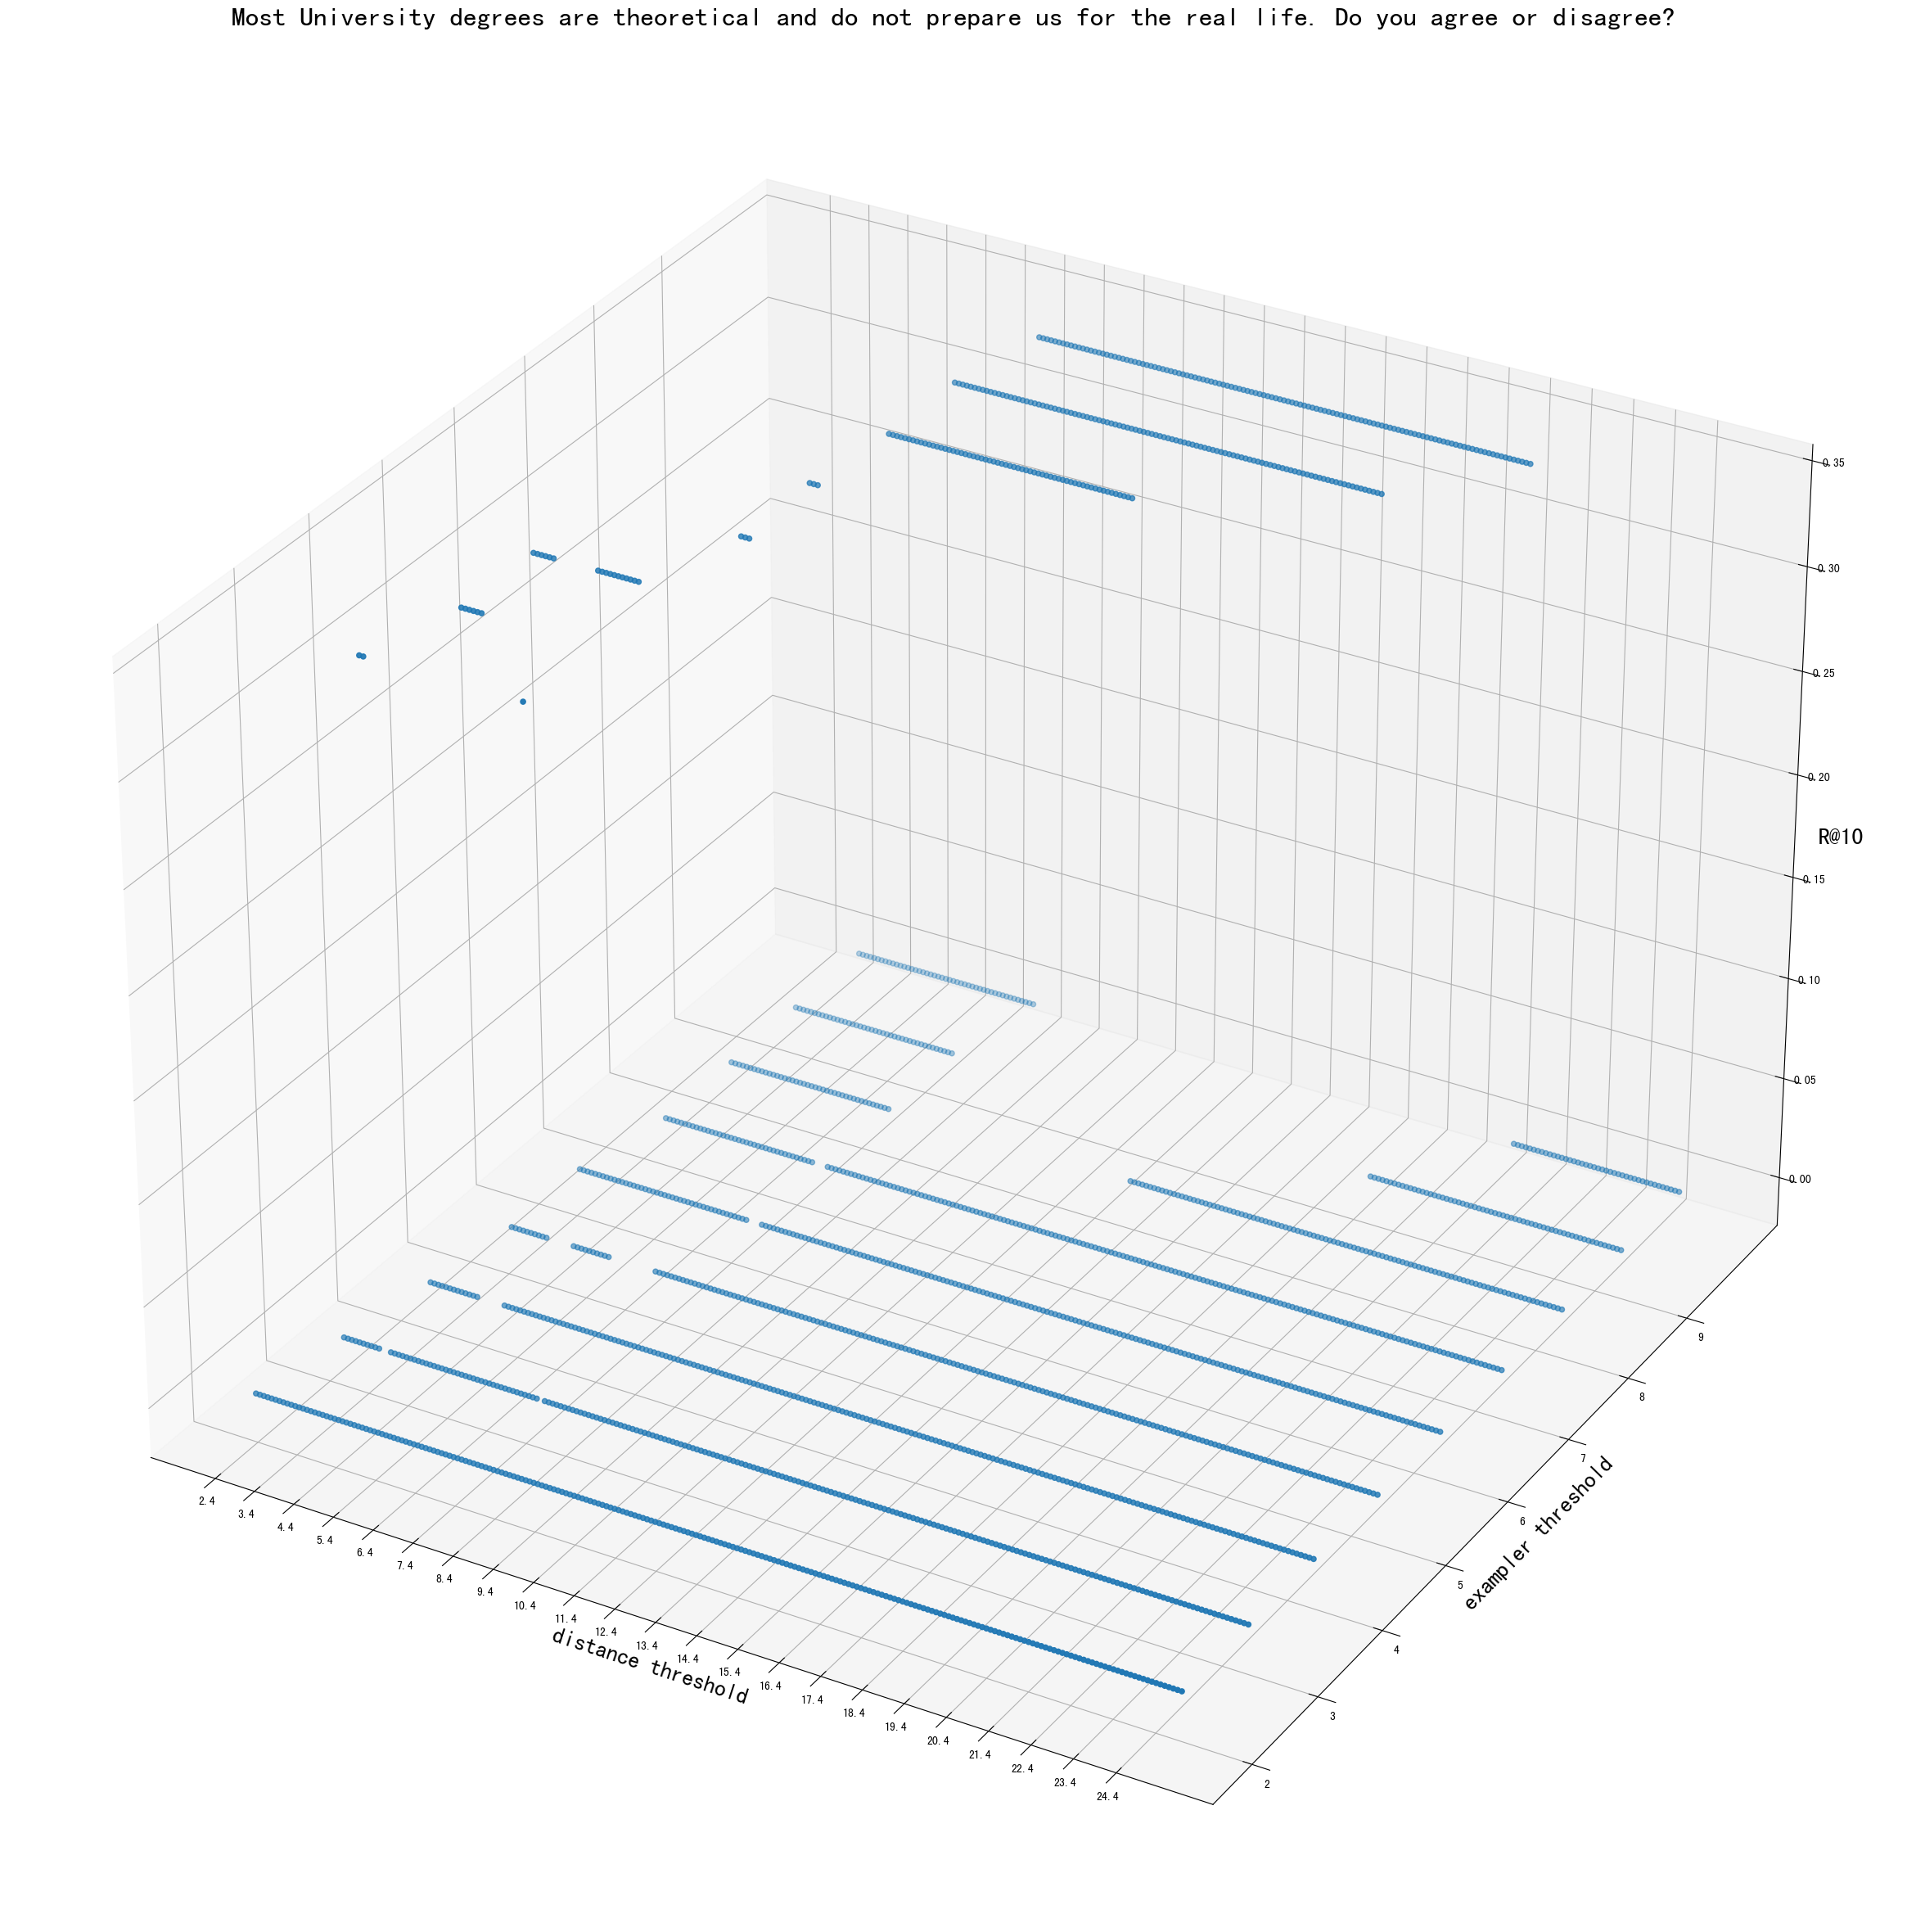
\includegraphics[width=1.0\linewidth]{MostUniversityDegreesAreTheoreticalAndDoNotPrepareUsForTheRealLifeDoYouAgreeOrDisagree_.png}
  \caption{变化趋势 (Topic:Most University degrees are theoretical and do not prepare us for the real life. Do you agree or disagree)}
  \label{framework}
\end{figure*}

% Table generated by Excel2LaTeX from sheet 'Sheet1'
\begin{table}[htbp]
  \centering
  \begin{tabular}{c|c|c|c|c|c}
    \hline
    \multicolumn{2}{c|}{} & \textbf{R@10} & \textbf{R@15} & \textbf{R@20} & \textbf{R@50} \\
    \hline
    \multicolumn{2}{c|}{\textbf{baseline}} & 0.4774  & 0.5109  & 0.5715  & 0.7148  \\
    \hline
    \multicolumn{2}{c|}{\textbf{tfidf}} & 0.3272  & 0.4267  & 0.4472  & 0.6292  \\
    \hline
    \multicolumn{2}{c|}{\textbf{doc2vec}} & 0.4471  & 0.4752  & 0.5540  & 0.7094  \\
    \hline
    \multirow{2}[0]{*}{\textbf{分类模型}} & \textbf{habilstm} & 0.5933  & 0.6062  & 0.6062  & 0.7184  \\
    & \textbf{bert} & \textcolor[rgb]{ 1,  0,  0}{\textbf{0.6062 }} & 0.6365  & 0.6971  & 0.8200  \\
    \hline
    \multirow{2}[0]{*}{\textbf{生成模型}} & \textbf{lstmabs} & 0.3068  & 0.3706  & 0.4221  & 0.6328  \\
    & \textbf{bertabs} & 0.5456  & 0.5608  & 0.5911  & 0.8057  \\
    \hline
  \end{tabular}%
  \caption{聚类方案二(one-class)指标对比}
  \label{tab:addlabel}%
\end{table}%

% Table generated by Excel2LaTeX from sheet '3.0划分(Accuracy)'
\begin{table}[htbp]
  \centering
  \begin{tabular}{c|c|c|c|c}
    \hline
    & \textbf{R@10} & \textbf{R@15} & \textbf{R@20} & \textbf{R@50} \\
    \hline
    \textbf{epsilon-SVR} & 0.3096  & 0.3652  & 0.4495  & 0.6571  \\
    \hline
    \textbf{ nu-SVR} & \textcolor[rgb]{ 1,  0,  0}{\textbf{0.3109 }} & 0.3695  & 0.4539  & 0.6790  \\
    \hline
  \end{tabular}%
  \caption{SVR分数排序方案指标对比}
  \label{tab:addlabel}%
\end{table}%


\end{CJK}
\end{document}

% include your own bib file like this:


%\begin{thebibliography}{}

%\bibitem[\protect\citename{Aho and Ullman}1972]{Aho:72}
%Alfred~V. Aho and Jeffrey~D. Ullman.
%\newblock 1972.
%\newblock {\em The Theory of Parsing, Translation and Compiling}, volume~1.
%\newblock Prentice-{Hall}, Englewood Cliffs, NJ.

%\bibitem[\protect\citename{{American Psychological Association}}1983]{APA:83}
%{American Psychological Association}.
%\newblock 1983.
%\newblock {\em Publications Manual}.
%\newblock American Psychological Association, Washington, DC.

%\bibitem[\protect\citename{{Association for Computing Machinery}}1983]{ACM:83}
%{Association for Computing Machinery}.
%\newblock 1983.
%\newblock {\em Computing Reviews}, 24(11):503--512.

%\bibitem[\protect\citename{Chandra \bgroup et al.\egroup }1981]{Chandra:81}
%Ashok~K. Chandra, Dexter~C. Kozen, and Larry~J. Stockmeyer.
%\newblock 1981.
%\newblock Alternation.
%\newblock {\em Journal of the Association for Computing Machinery},
%  28(1):114--133.

%\bibitem[\protect\citename{Gusfield}1997]{Gusfield:97}
%Dan Gusfield.
%\newblock 1997.
%\newblock {\em Algorithms on Strings, Trees and Sequences}.
%\newblock Cambridge University Press, Cambridge, UK.

%\bibitem[\protect\citename{Rasooli and Tetreault}2015]{rasooli-tetrault-2015}
%Mohammad~Sadegh Rasooli and Joel~R. Tetreault. 2015.
%\newblock {Yara parser: {A} fast and accurate dependency parser}.
%\newblock \emph{Computing Research Repository}, arXiv:1503.06733.
%\newblock Version 2.

%\bibitem[\protect\citename{Borschinger and Johnson}2011]{borsch2011}
%Benjamin Borschinger and Mark Johnson. 2011.
%\newblock A particle filter algorithm for {B}ayesian wordsegmentation.
%\newblock In \emph{Proceedings of the Australasian Language Technology Association %Workshop 2011}, pages 10--18, Canberra, Australia.

%\end{thebibliography}

